\documentclass{article}

\usepackage{../mathclub}

\title{Gambling} 
\author{}
\date{April 4, 2022}

\begin{document}

\section{Introduction}

Today we discuss concepts which arise from gambling situations, but which have applications throughout probability, statistics, and elsewhere. Even if a strategy is useless to the gambler, it can be a very powerful tool in the hands of a mathematician.

References: PSTAT 160AB, Matt Baker's blog, \emph{Random Walks and Electric Networks} by Doyle and Snell, \emph{Exercises in Probability} by Cacoullos, and <randomservices.org>.

\begin{exercise}
The game of ``craps'' is played as follows. The gambler throws two dice. If at first throw he gets $7$ or $11$ he wins, and if he gets $2$, $3$, or $12$ he loses. For each of the other sums the gambler continues throwing the two dice until he wins with a $7$ or he loses with the outcome of the first throw. What is the probability of the gambler winning?
\end{exercise}

\begin{exercise}
In a game of tossing a fair coin (two gamblers pick a side of a fair coin and toss it), the first one to $n$ successes (heads or tails) wins. Show that the game is fair (each gambler has a probability of winning equal to $1/2$). Suppose that the game was interrupted when the first gambler had won $k$ tosses and the second gambler had won $m$ tosses, where $0\leqs k,m<n$. Calculate for each gambler the probability of winning if the game is continued. 
\end{exercise}

\section{Gambler's Ruin and Martingales}

Consider the setting of gambler's ruin. A gambler begins with $x$ dollars, and bets $\$ 1$ at each round. Suppose that with probability $p$ (respectively, $1-p$) the gambler wins (respectively, loses). The gambler will only leave if she reaches $N$ dollars, in which case she stops playing and collects her winnings, or if she loses all her money. 

We can (and should) reinterpret this scenario as a ``random walk'' on the set $S=\{0,1,\dots,N\}$. At any given integer $x$ (other $0$ or $N$) we move to $x+1$ with probability $p$ or $x-1$ with probability $1-p$. The walk ends when we get to $0$ or $N$.

\begin{exercise}
Call a function $f:S\to \RR$ \emph{harmonic} if it satisfies the ``mean-value property'' 
\[f(x)=\frac{f(x-1)+f(x+1)}{2}\] for all $x\in \{1,\dots,N-1\}$. Prove that the harmonic functions are closed under addition and scalar multiplication. 
\end{exercise}

\begin{exercise}
Let $p(x)$ denote the probability that, starting with $x$ dollars, the gambler will win (so the probability of ``ruin,'' or bankruptcy, is $1-p(x)$). We can think of $p$ as a function $S\to [0,1]$. Prove that 
\begin{enumerate}[label=\textbf{(\alph*)}]
    \item $p(0)=0$
    \item $p(N)=1$
    \item $p(x) = \frac{p(x-1)+p(x+1)}{2}$
\end{enumerate}
Deduce that the expected value $e(x)$ of the final fortune (given that she starts at $x$) of the gambler is given by a harmonic function.
\end{exercise}

\begin{exercise}
A nice exercise for those of you who know your physics. Consider a circuit with a $1$-volt battery and $N$ resistors connected in series, as shown. We select points $0,1,\dots,N$ between the resistors. Let $v(x)$ denote the voltage at the point $x$. Prove that $v(x)$ is harmonic.
\end{exercise}

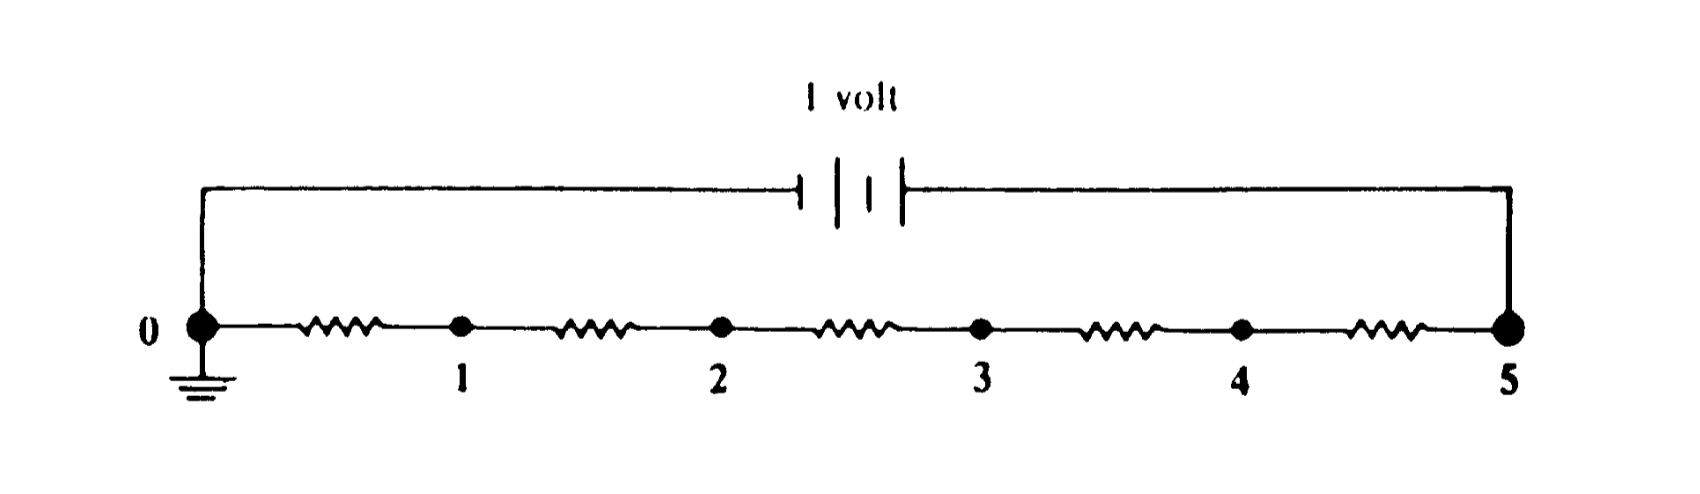
\includegraphics[scale=0.5]{Pics/Screen Shot 2022-04-04 at 6.51.21 AM.png}

\begin{remark}
We can choose our convention so that $v(0)=0$ and $v(N)=1$. Hence $v(x)$ and $p(x)$ are two harmonic functions which agree at the boundary values $0$ and $N$. We can invoke a general ``uniqueness theorem'' for harmonic functions to deduce that $v(x)=p(x)=x/N$ identically. 
\end{remark}

\begin{exercise}
Assume now that $p=\frac{1}{2}$. Prove that the game is \emph{fair}, namely that for any $x$ the expected amount of dollars you have in the next round, given that you currently have $x$, equals $x$. 
\end{exercise}

\begin{theorem}[Martingale Stopping Theorem]
A fair game that is stopped at a random time will remain fair to the end of the game if it is assumed that there is a finite amount of money in the world and a player must stop if he wins all this money or goes into debt by this amount.
\end{theorem}

What this means to us is that, in a fair game, the expected final fortune is equal to what we started with, i.e. $e(x)=x$. 

\begin{exercise}
Still in the case $p=\frac{1}{2}$, calculate the expected final fortune as a function of $x$.
\end{exercise}

\begin{exercise}
Now assume $p\neq \frac{1}{2}$. Then the game as it stands is not fair, but if we \emph{interpret} the fortune at point $x$ to be $(\frac{1-p}{p})^x$, then the game becomes fair. Derive a formula for the expected final fortune of the gambler.
\end{exercise}

\begin{remark}
The theory can get quite sophisticated, so I will stop here. Martingales have lots of applications throughout probability, statistics, combinatorics, finance, and potential theory. Some of these include Wald's equation, the fundamental theorem of asset pricing, the secretary problem, and elegant proofs of a lot of well-known theorems. 
\end{remark}

\end{document}